% Compile with: latexmk -lualatex main.tex   (LuaLaTeX is required for the Bengali text; font: Noto Sans Bengali)
\documentclass[journal]{IEEEtran}
\usepackage{fontspec}
\usepackage{amsmath}
\usepackage{graphicx}
\usepackage{booktabs}
\usepackage{multirow}
\usepackage{array}
\usepackage{url}
\usepackage{cite}
\usepackage{hyperref}
\newfontfamily\bnfont[Script=Bengali]{Noto Sans Bengali}
\newcommand{\bn}[1]{{\bnfont #1}}
\newcommand{\pmstd}[2]{#1$\pm$#2}
\graphicspath{{figures/}}
\hypersetup{hidelinks}

\begin{document}

\title{Beyond the Single Split: A Reproducible Benchmark of Bengali Book Review Sentiment Classification with Explanations and Label-Noise Analysis}

\author{Anonymous Authors}

\markboth{Manuscript draft}{Anonymous: Bengali Book Review Sentiment Classification}

\maketitle

\begin{abstract}
Bengali book review sentiment classification remains challenging because of spelling variation, informal language, and limited annotated data. This study benchmarks twelve trainable-embedding recurrent and attention-based models, nineteen classical TF-IDF classifiers, and pretrained transformers (BanglaBERT, BanglaBERT-large, XLM-R and multilingual BERT) for binary sentiment prediction. A dataset of 2{,}009 unique reviews (1{,}029 negative and 980 positive), called BBR-2009, was reconstructed from the Mendeley Bengali Book Reviews corpus and BanglaBook, and all models were evaluated with stratified five-fold cross-validation (five seeds for the recurrent models, three for the transformers). The recurrent models reached at most 81.08\% mean accuracy (BiLSTM with attention), with single-fold accuracies spanning 13 points, whereas fine-tuned BanglaBERT reached \pmstd{93.84}{1.10}\% over three seeds, BanglaBERT-large \pmstd{93.81}{1.04}\%, and their probability-averaging ensemble \pmstd{94.23}{0.82}\% (a gain that is not statistically significant). After hyper-parameter tuning, XLM-R and multilingual BERT reached \pmstd{91.31}{1.12}\% and \pmstd{86.83}{1.54}\%. On the Mendeley corpus BanglaBERT reached \pmstd{96.72}{1.19}\% against 94.24\% for the strongest TF-IDF baseline; on the Rokomari corpus it reached \pmstd{90.60}{0.72}\%. On the official three-class BanglaBook benchmark our best result (a validation-selected ensemble, 0.927 weighted F1) remains 0.6 points below the published 0.933. SHAP explanations pass a deletion-based faithfulness check, and an error analysis shows that 62\% of model errors are confident disagreements concentrated in the rating-derived source; a blind LLM-assisted audit supports the view that many of them are label errors. We release the dataset construction, fold assignments and code.
\end{abstract}

\begin{IEEEkeywords}
Bengali sentiment analysis, book reviews, BanglaBERT, label noise, cross-validation, explainability, SHAP.
\end{IEEEkeywords}

\IEEEpeerreviewmaketitle

\section{Introduction}
Bengali is a widely spoken language with a growing volume of reader-generated reviews on digital platforms. Such reviews contain useful signals about readers' preferences, satisfaction, and criticism, but examining them manually at scale is difficult. Online Bengali reviews include informal wording, spelling variants, punctuation differences, emoji and variable length, which makes reliable sentiment identification difficult, especially when labelled resources are limited. Traditional classifiers use sparse lexical features; recurrent neural networks (RNNs) process sequences of word representations; and pretrained transformers transfer knowledge learned from large corpora.

Published results on Bengali book reviews are hard to compare. They are usually obtained on a single train/test split of a small corpus, with weak baselines, and sometimes with labels derived from star ratings. A single 400-review test set already has a 95\% confidence interval of about $\pm 2$ percentage points at 95\% accuracy. In our own cross-validation the best recurrent model scores anywhere between 72.6\% and 85.8\% on different folds, so the figure one reports depends heavily on which reviews are held out.

This paper therefore makes the following contributions.
\begin{enumerate}
\item A cross-validated benchmark (stratified five-fold, 3--5 seeds) of twelve recurrent configurations, nineteen classical classifiers and four pretrained transformers on a 2{,}009-review Bengali book review set, and on the Mendeley and Rokomari corpora, with statistical tests and calibration.
\item Evidence that single-split figures are unstable (fold accuracies of one model span 13 points; recurrent models 73--81\% on average), that a simple TF-IDF Naive Bayes already reaches 94.2\% on the public Mendeley reviews, far above the 84\% reported earlier on a larger corpus, and that language-specific pretraining (BanglaBERT) is the decisive factor.
\item A label-noise analysis: confident model errors concentrate in rating-derived labels (8.6\% of BanglaBook-originated reviews against 1.3\% of Mendeley reviews), and a blind re-annotation audit indicates that many of them are label errors.
\item An extended SHAP analysis with a deletion-based faithfulness test, cross-source transfer experiments, and an honest comparison with the official BanglaBook and Rokomari benchmarks, where we do \emph{not} claim state-of-the-art results.
\item A public release of the dataset reconstruction, fold assignments and a datasheet.
\end{enumerate}
The remainder of the paper reviews related work (Section~\ref{sec:related}), describes the data and methods (Section~\ref{sec:method}), reports the results (Section~\ref{sec:results}), and presents the discussion, limitations and conclusion.

\section{Related Work}\label{sec:related}
Early sentiment classifiers relied on Naive Bayes, logistic regression and support vector machines over hand-crafted features such as TF-IDF, and struggled with context and long-range dependencies \cite{pang2002}. Recurrent networks learn order-dependent features \cite{mikolov2010}; LSTM and GRU gating mitigates long-term dependency problems \cite{hochreiter1997,cho2014}; bidirectional variants use both directions \cite{schuster1997}; and attention lets a model weight informative words \cite{bahdanau2015,wang2016}. Dense word representations underlie most neural sentiment models \cite{mikolov2013}. The Transformer \cite{vaswani2017} and BERT-style pretraining \cite{devlin2019} changed this picture, and BanglaBERT \cite{bhattacharjee2022} is an ELECTRA-based model pretrained on a large Bengali corpus. XLM-R \cite{conneau2020} is a multilingual alternative.

For Bengali, Islam \emph{et al.}\ used multilingual BERT transfer learning \cite{islam2020}, Hasan \emph{et al.}\ compared classical and neural models \cite{hasan2020}, and Bhowmick and Jana studied transformer models \cite{bhowmick2021}. For book reviews, Hossain \emph{et al.}\ applied multinomial Naive Bayes to their own 2,000-review corpus (84\%) \cite{hossain2020}; Sarker \emph{et al.}\ compared LSTM variants and transformers on Rokomari reviews and obtained a weighted F1 of 88.95\% with XLM-R \cite{sarker2022}; and BanglaBook \cite{kabir2023} provides 158{,}065 reviews labelled from star ratings, where BanglaBERT-large reaches about 0.93 weighted F1 on the three-class split. Ensembles of complementary models are a standard way to reduce variance \cite{dietterich2000}.

We found no work that (i) evaluates Bengali book review classifiers under repeated cross-validation with significance tests, (ii) quantifies how rating-derived labels inflate or deflate reported accuracy, or (iii) tests the faithfulness of token attributions on this task. These are the gaps addressed here.

\section{Data and Methods}\label{sec:method}
\subsection{Datasets}
The primary dataset, BBR-2009, contains 2{,}009 unique Bengali book reviews: 980 positive (label 1) and 1{,}029 negative (label 0). It combines the Mendeley Bengali Book Reviews corpus (1{,}414 reviews after near-duplicate removal; 947 positive, 467 negative; manual labels; CC BY 4.0) with 595 reviews from BanglaBook \cite{kabir2023} (562 negative and 33 positive; star ratings 1--2 mapped to negative and 5 to positive, Bengali script only, at least three words; CC BY-NC-SA 4.0). The merged corpus is a reconstruction from these public sources, built for this study; it is not a continuation of an earlier private file. We release the review text, labels, source flags and the exact fold assignments with a datasheet, for non-commercial use. Because the BanglaBook portion is almost entirely negative, source and label are partly confounded, so accuracy is also reported per source. The Mendeley corpus alone (1{,}442 unique reviews) and the Rokomari corpus \cite{sarker2022} (positive and negative reviews only) are evaluated separately. A cleaned external Rokomari set (5{,}277 reviews: 2{,}670 positive, 2{,}607 negative; neutral reviews removed, reviews present in BBR-2009 excluded) is used for zero-shot external testing.

\begin{figure}[t]
\centering
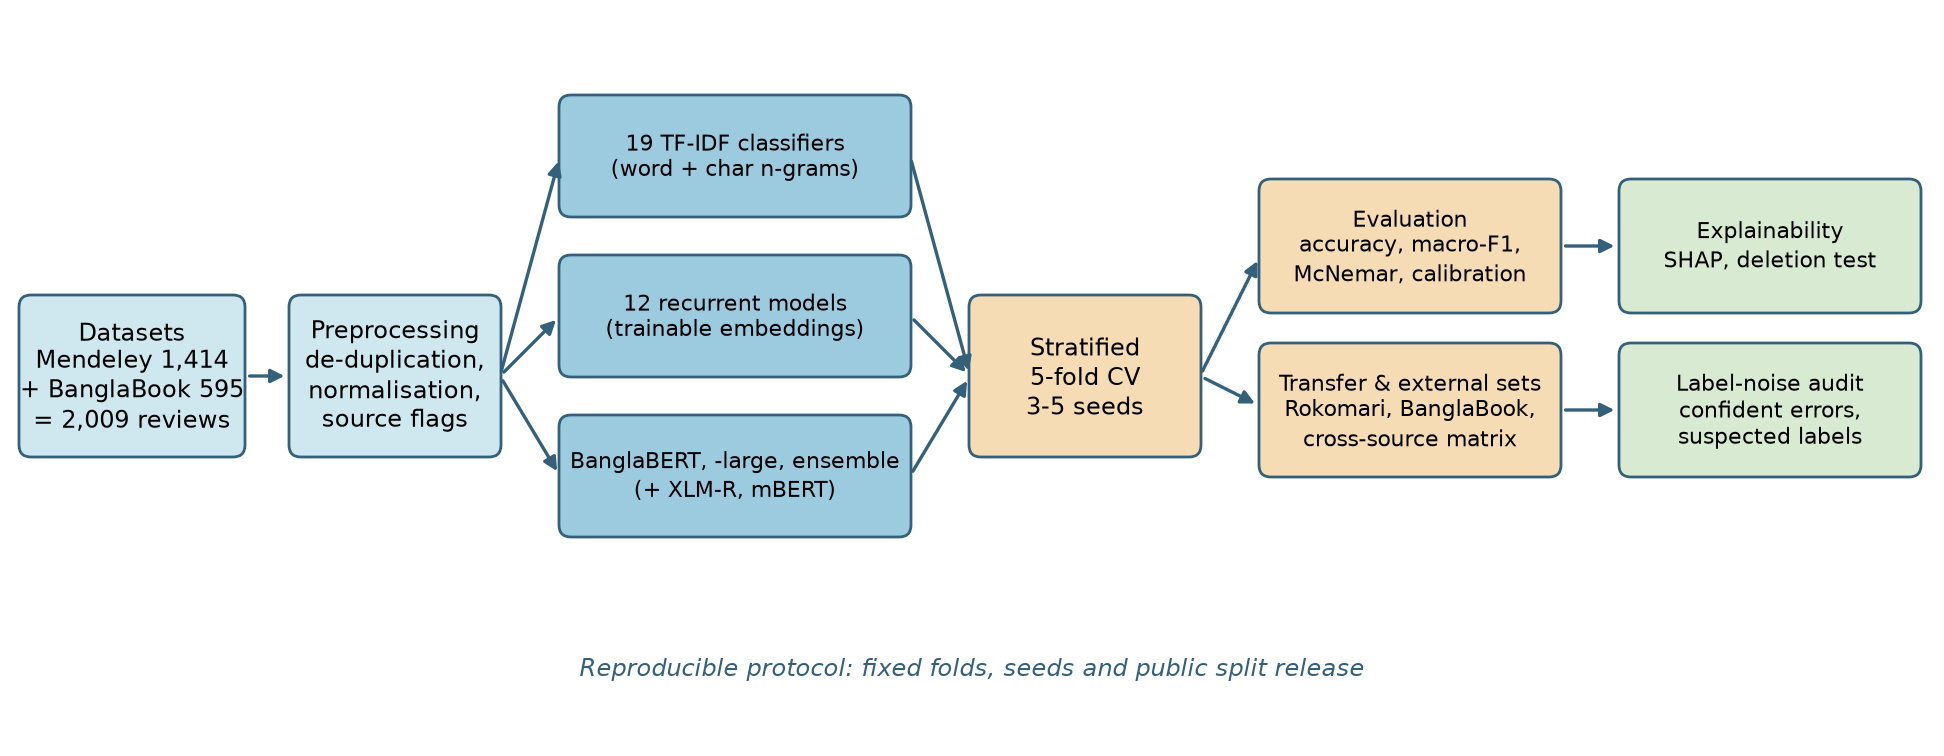
\includegraphics[width=\columnwidth]{fig3_pipeline.png}
\caption{Experimental pipeline: classical, recurrent and transformer models are evaluated under repeated stratified cross-validation, followed by transfer, explainability and label-noise analyses.}
\label{fig:pipeline}
\end{figure}

\subsection{Preprocessing and Representations}
Reviews were stripped of unnecessary characters and punctuation while preserving Bengali Unicode text. For the recurrent models, tokens were integer-encoded with a 15{,}000-word vocabulary and an out-of-vocabulary token, padded or truncated to 150 tokens, and passed to a trainable 128-dimensional embedding layer. The transformers use their own sub-word tokenizers (maximum length 128). The classical models use word (1--2-gram) and character (2--5-gram) TF-IDF features; dense-input models use a 200-component truncated SVD.

\subsection{Models and Training}
\textbf{Recurrent models.} Twelve configurations (RNN, GRU, LSTM; unidirectional or bidirectional; with or without additive attention) were trained with packed variable-length sequences, Adam (learning rate $10^{-3}$), gradient clipping at 1.0, dropout 0.3, balanced class weights, and early stopping on a 10\% validation split of each training fold (patience 4, at most 20 epochs), so test folds were never used for model selection.

\textbf{Classical models.} Nineteen classifiers were trained: logistic regression, linear and RBF SVM, $k$-NN, decision tree, random forest, extra trees, multinomial/Bernoulli/Gaussian Naive Bayes, LDA, QDA, XGBoost, LightGBM, CatBoost, gradient boosting, histogram gradient boosting, AdaBoost and an MLP.

\textbf{Transformers.} BanglaBERT \cite{bhattacharjee2022} was fine-tuned for four epochs with AdamW (learning rate $3\times10^{-5}$, batch size 16, maximum length 128, linear warm-up and decay, balanced class weights). BanglaBERT-large used learning rate $2\times10^{-5}$ and batch size 8. XLM-R base and multilingual BERT were tuned over learning rates $\{1,2,3,5\}\times10^{-5}$ and $\{4,6\}$ epochs on a tuning split taken from the training part of fold 0 of seed 0 (the fold-0 test part was never used), which selected $2\times10^{-5}$/6 epochs for XLM-R and $3\times10^{-5}$/6 epochs for mBERT. The ensemble averages the predicted probabilities of BanglaBERT and BanglaBERT-large.

\subsection{Evaluation}
All models used stratified five-fold cross-validation (about 1{,}607 training and 402 test reviews per fold): five seeds for the recurrent models, three seeds for the transformers and for the classical models on BBR-2009, three seeds on Mendeley, and one seed for the Rokomari corpus. We report accuracy and macro-averaged precision, recall and F1 as mean $\pm$ standard deviation over runs. Paired comparisons use the Wilcoxon signed-rank test over runs and McNemar's test \cite{mcnemar1947} on pooled out-of-fold predictions; calibration is measured with the expected calibration error (ECE, 10 bins) \cite{guo2017}. Explanations use SHAP \cite{lundberg2017} with a text masker.

\begin{table}[t]
\centering
\caption{Dataset and training configuration.}
\label{tab:config}
\small
\begin{tabular}{ll}
\toprule
Parameter & Value \\
\midrule
Training / test samples & $\approx$1{,}607 / 402 per fold \\
Vocabulary size (RNN) & 15{,}000 \\
Maximum sequence length & 150 (RNN) / 128 (transformers) \\
Embedding dimension (RNN) & 128 \\
Batch size / maximum epochs & 32 / 20 (RNN); 16 / 4 (BERT) \\
Early-stopping patience (RNN) & 4 \\
Class weights & balanced, from training labels \\
\bottomrule
\end{tabular}
\end{table}

\section{Results}\label{sec:results}
\subsection{Recurrent Models}
Table~\ref{tab:rnn} lists the cross-validated results of the twelve recurrent models (25 runs each) together with BanglaBERT. With the corrected training procedure (packed sequences, gradient clipping, validation-based early stopping) no configuration collapsed to a single class, as some unidirectional recurrent models can do without these safeguards. Attention improved five of the six cell/direction combinations, and the best recurrent model was BiLSTM with attention (\pmstd{81.08}{3.75}\%), followed by BiGRU with attention (\pmstd{80.62}{4.05}\%). Variation across folds is large (standard deviations of 3.6--6.7 points), and the same BiLSTM with attention scores anywhere between 72.6\% and 85.8\% on different folds. BanglaBERT reached \pmstd{93.84}{1.10}\% accuracy with much lower variance.

\begin{table}[t]
\centering
\caption{Five-fold cross-validated performance on BBR-2009 (recurrent: 25 runs; BanglaBERT: 15 runs). Accuracy is mean $\pm$ std; other columns are macro-averaged means (\%).}
\label{tab:rnn}
\small
\begin{tabular}{lcccc}
\toprule
Model & Accuracy & Precision & Recall & F1 \\
\midrule
RNN & \pmstd{73.57}{6.20} & 74.00 & 73.60 & 73.43 \\
BiRNN & \pmstd{75.11}{4.82} & 75.47 & 75.11 & 75.00 \\
GRU & \pmstd{78.06}{6.72} & 78.57 & 78.14 & 77.94 \\
BiGRU & \pmstd{79.88}{4.81} & 80.24 & 79.93 & 79.82 \\
LSTM & \pmstd{79.54}{4.87} & 80.32 & 79.65 & 79.40 \\
BiLSTM & \pmstd{80.43}{4.33} & 80.86 & 80.48 & 80.36 \\
RNN + Attention & \pmstd{78.33}{4.18} & 78.91 & 78.39 & 78.20 \\
BiRNN + Attention & \pmstd{79.41}{4.02} & 80.10 & 79.48 & 79.29 \\
GRU + Attention & \pmstd{79.45}{3.58} & 80.25 & 79.57 & 79.31 \\
BiGRU + Attention & \pmstd{80.62}{4.05} & 81.31 & 80.69 & 80.50 \\
LSTM + Attention & \pmstd{78.78}{4.35} & 79.34 & 78.81 & 78.66 \\
BiLSTM + Attention & \pmstd{81.08}{3.75} & 81.63 & 81.13 & 80.99 \\
\midrule
BanglaBERT (base) & \pmstd{93.84}{1.10} & 93.93 & 93.90 & 93.84 \\
\bottomrule
\end{tabular}
\end{table}

\subsection{Transformers, Classical Models and Published Baselines}
Table~\ref{tab:main} compares the models on three datasets. On the Mendeley corpus, BanglaBERT (\pmstd{96.72}{1.19}\% over 15 folds) exceeded the strongest classical baseline, multinomial Naive Bayes (\pmstd{94.24}{1.72}\%), by 2.5 points and was higher on every fold of seed 0 (minimum fold-wise gain 1.0 points). The 84\% reported for Naive Bayes in \cite{hossain2020} comes from the authors' own 2,000-review corpus, of which only 1,443 reviews are public, so the comparison is indicative only. On the Rokomari corpus BanglaBERT reached \pmstd{90.60}{0.72}\% accuracy (macro-F1 90.47\%) against 88.42\% for linear SVM. The published 88.95\% weighted F1 of XLM-R \cite{sarker2022} was obtained with a different split; the original shuffle in the authors' code is unseeded, so their exact split cannot be reproduced. We therefore followed their protocol (positive and negative reviews of at most 300 words, stratified 80/10/10 split) with three random shuffles: weighted F1 was 89.21\%, 90.35\% and 90.35\% (mean $89.97\pm0.66$; 519 test reviews each). This is 1.0 point above the published value, but with a different split and a test set of this size the difference is within the shuffle-to-shuffle variation and is not evidence of superiority.

On BBR-2009, BanglaBERT (\pmstd{93.84}{1.10}\%) and BanglaBERT-large (\pmstd{93.81}{1.04}\%) were indistinguishable over three seeds (paired Wilcoxon $p=0.89$), and their ensemble reached \pmstd{94.23}{0.82}\%; this gain of 0.4 points over the base model is smaller than the fold-to-fold deviation and not significant ($p=0.16$). In an earlier single-seed run the large model appeared better (94.28\% vs 93.53\%), which was seed noise. Under the same protocol XLM-R base reached \pmstd{91.31}{1.12}\% after tuning (\pmstd{91.11}{1.12}\% with default settings) and multilingual BERT \pmstd{86.83}{1.54}\% (default \pmstd{86.53}{1.45}\%); the ordering BanglaBERT $>$ XLM-R $>$ mBERT held in every seed, so Bengali-specific pretraining was more useful than multilingual pretraining. XLM-R was only about one point above the best TF-IDF baseline (90.19\%), and mBERT was below it. Tuning changed the results by at most 0.3 points.

\begin{table*}[t]
\centering
\caption{Cross-validated accuracy (\%, mean $\pm$ std) on three datasets, with the best published results. BBR-2009 rows use three seeds (recurrent: five); Mendeley and Rokomari classical rows are as reported by the same protocol.}
\label{tab:main}
\small
\begin{tabular}{lccc}
\toprule
Method & Mendeley & BBR-2009 & Rokomari \\
\midrule
BanglaBERT (base) & \pmstd{96.72}{1.19} & \pmstd{93.84}{1.10} & \pmstd{90.60}{0.72} \\
BanglaBERT-large & -- & \pmstd{93.81}{1.04} & -- \\
Base + large ensemble & -- & \pmstd{94.23}{0.82} & -- \\
XLM-R base (tuned) & -- & \pmstd{91.31}{1.12} & -- \\
Multilingual BERT (tuned) & -- & \pmstd{86.83}{1.54} & -- \\
BiLSTM + attention (from scratch) & -- & \pmstd{81.08}{3.75} & -- \\
Linear SVM (TF-IDF) & \pmstd{93.55}{1.84} & \pmstd{90.19}{1.53} & \pmstd{88.42}{1.02} \\
Logistic regression & \pmstd{93.48}{1.69} & \pmstd{90.08}{1.66} & \pmstd{88.16}{0.94} \\
Multinomial NB & \pmstd{94.24}{1.72} & \pmstd{89.50}{1.67} & \pmstd{84.08}{1.52} \\
\midrule
Published best & 84.0 \cite{hossain2020} & n/a & 88.95 wF1 \cite{sarker2022} \\
\bottomrule
\end{tabular}
\end{table*}

\subsection{Ablation}
Table~\ref{tab:abl} reports a fine-tuning ablation of BanglaBERT over three seeds. Removing class weights or raising the learning rate to $5\times10^{-5}$ did not change the accuracy, while shortening the maximum length to 64 or reducing training to two epochs lowered it by 0.6--0.7 points, still within one standard deviation (93.13--93.86\%), so the result is not very sensitive to these choices.

\begin{table}[t]
\centering
\caption{Ablation of BanglaBERT fine-tuning (BBR-2009, 3 seeds $\times$ 5 folds).}
\label{tab:abl}
\small
\begin{tabular}{lc}
\toprule
Variant & Accuracy (\%) \\
\midrule
Default ($3\times10^{-5}$, length 128, 4 epochs, class weights) & \pmstd{93.84}{1.10} \\
Learning rate $5\times10^{-5}$ & \pmstd{93.86}{1.31} \\
No class weights & \pmstd{93.83}{1.27} \\
Maximum length 64 & \pmstd{93.26}{1.42} \\
2 epochs & \pmstd{93.13}{1.21} \\
\bottomrule
\end{tabular}
\end{table}

\subsection{Statistical Tests, Calibration and Error Analysis}
McNemar's test showed that the ensemble was significantly more accurate than the best classical model (linear SVM) in every seed ($p<10^{-8}$; in seed 0, 130 reviews were correct only for the ensemble and 48 only for the SVM), but significantly better than the base model in only one of three seeds ($p=0.03$, 0.87, 0.67). The ECE was 0.047 (base), 0.057 (large) and 0.041 (ensemble). Errors were more frequent for BanglaBook-originated reviews (12.1\% vs 2.8\%) and for negative reviews (7.5\% vs 3.5\%); the presence of a negation word did not increase the error rate (4.7\% vs 5.9\%), and there was no clear trend with length (4.2--7.0\% across quartiles). Out-of-fold confusion matrices (seed 0, Fig.~\ref{fig:cm}) show 130 errors for the base model (95 negative and 35 positive reviews misclassified) and 115 for the large model (81 and 34).

\begin{figure}[t]
\centering
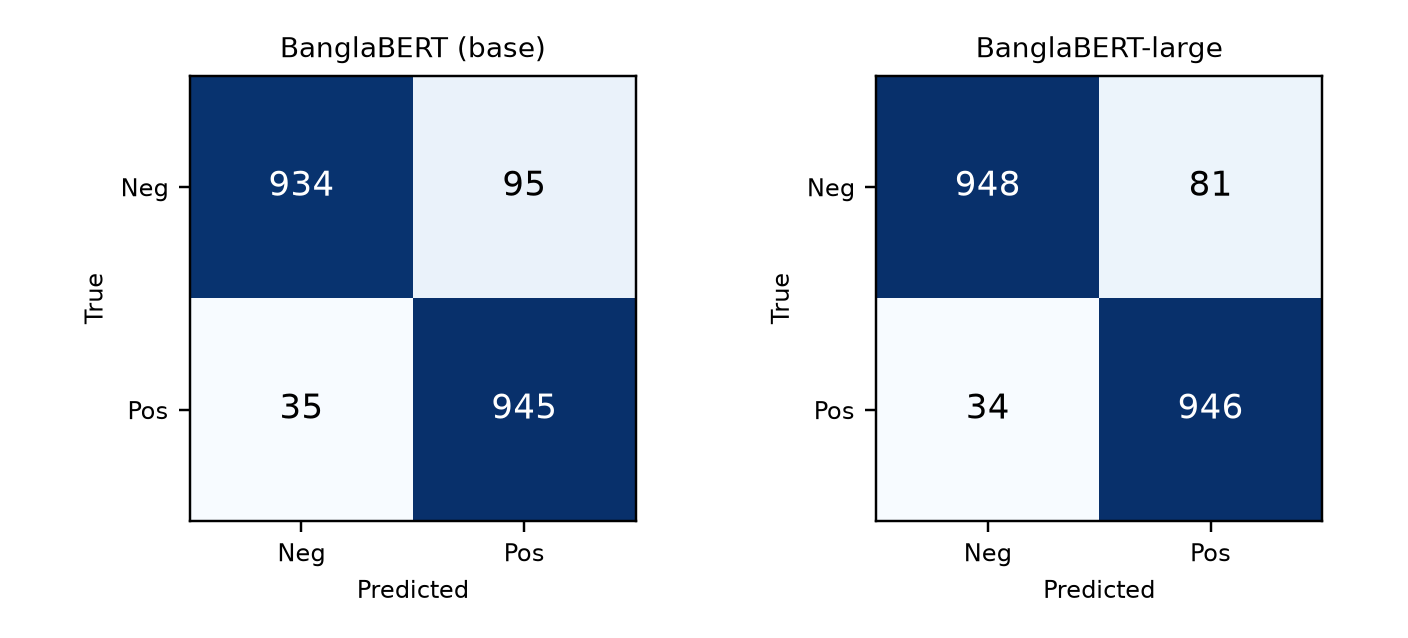
\includegraphics[width=\columnwidth]{fig4_confusion.png}
\caption{Out-of-fold confusion matrices of BanglaBERT (left) and BanglaBERT-large (right) on BBR-2009 (five-fold CV, seed 0).}
\label{fig:cm}
\end{figure}

\subsection{Label Noise}
Pooling out-of-fold predictions over three seeds and both model sizes, 111 of 2{,}009 reviews (5.5\%) were misclassified by the ensemble, and 69 of these errors (62\%) were made with a predicted probability above 0.9. Such confident disagreements are candidates for mislabelled data. They concentrate in the rating-derived source: 51 of 595 BanglaBook-originated reviews (8.6\%) against 18 of 1{,}414 Mendeley reviews (1.3\%).

\textbf{Blind re-annotation audit.} To test whether these are real label errors, the 69 suspected and 131 randomly drawn reviews were shuffled, stripped of their labels and re-labelled as positive, negative or unclear by a single large-language-model annotator from the review text only. This is an LLM-assisted audit by one annotator, \emph{not} a human annotation study, and it should be replicated with independent human annotators. 28 reviews were judged unclear (13 random, 15 suspected) and excluded. On the 118 labelled random reviews the annotator agreed with the dataset label in 96.6\% of cases (Cohen's $\kappa=0.93$; 100\% on Mendeley-originated and 87.1\% on BanglaBook-originated reviews), so the annotator does not simply contradict the data. On the 54 labelled suspected reviews agreement was only 25.9\% ($\kappa=0.00$): 39 of the 43 reviews labelled negative in the dataset were judged positive, and agreement was 9.8\% for BanglaBook-originated suspected reviews against 76.9\% for Mendeley-originated ones. Many suspected errors are therefore likely rating-derived labels that contradict the review text, which supports the view that star ratings are a noisy proxy for sentiment and that accuracy on the BanglaBook-originated portion is pessimistic.

\subsection{Explainability}
SHAP values \cite{lundberg2017} were first computed for 60 held-out reviews (Fig.~\ref{fig:shap}) and then for all 402 held-out reviews of an 80/20 split (Fig.~\ref{fig:shap402}). Negative evidence comes from words such as \bn{বাজে} (bad), \bn{দুর্বল} (weak), \bn{বিরক্তিকর} (annoying) and \bn{ফালতু} (worthless), and positive evidence from \bn{চমৎকার} (excellent), \bn{অসাধারণ} (extraordinary), \bn{দারুণ} (great) and \bn{সেরা} (best), i.e.\ sentiment-bearing words. A few frequent function words and sub-word pieces also appear, indicating some dataset-specific cues. As a faithfulness check, the $k$ highest-SHAP tokens of each review were deleted and the drop in the predicted-class probability was compared with deleting $k$ random tokens: 0.120 vs 0.024 ($k=1$), 0.324 vs 0.095 ($k=3$) and 0.444 vs 0.150 ($k=5$); SHAP-selected tokens are therefore three to five times more influential than random ones. Accuracy also differs by source: 95.5\% (negative) and 97.3\% (positive) on Mendeley-originated reviews against 86.8\% and 72.7\% on BanglaBook-originated negatives and positives (33 positives only).

\begin{figure}[t]
\centering
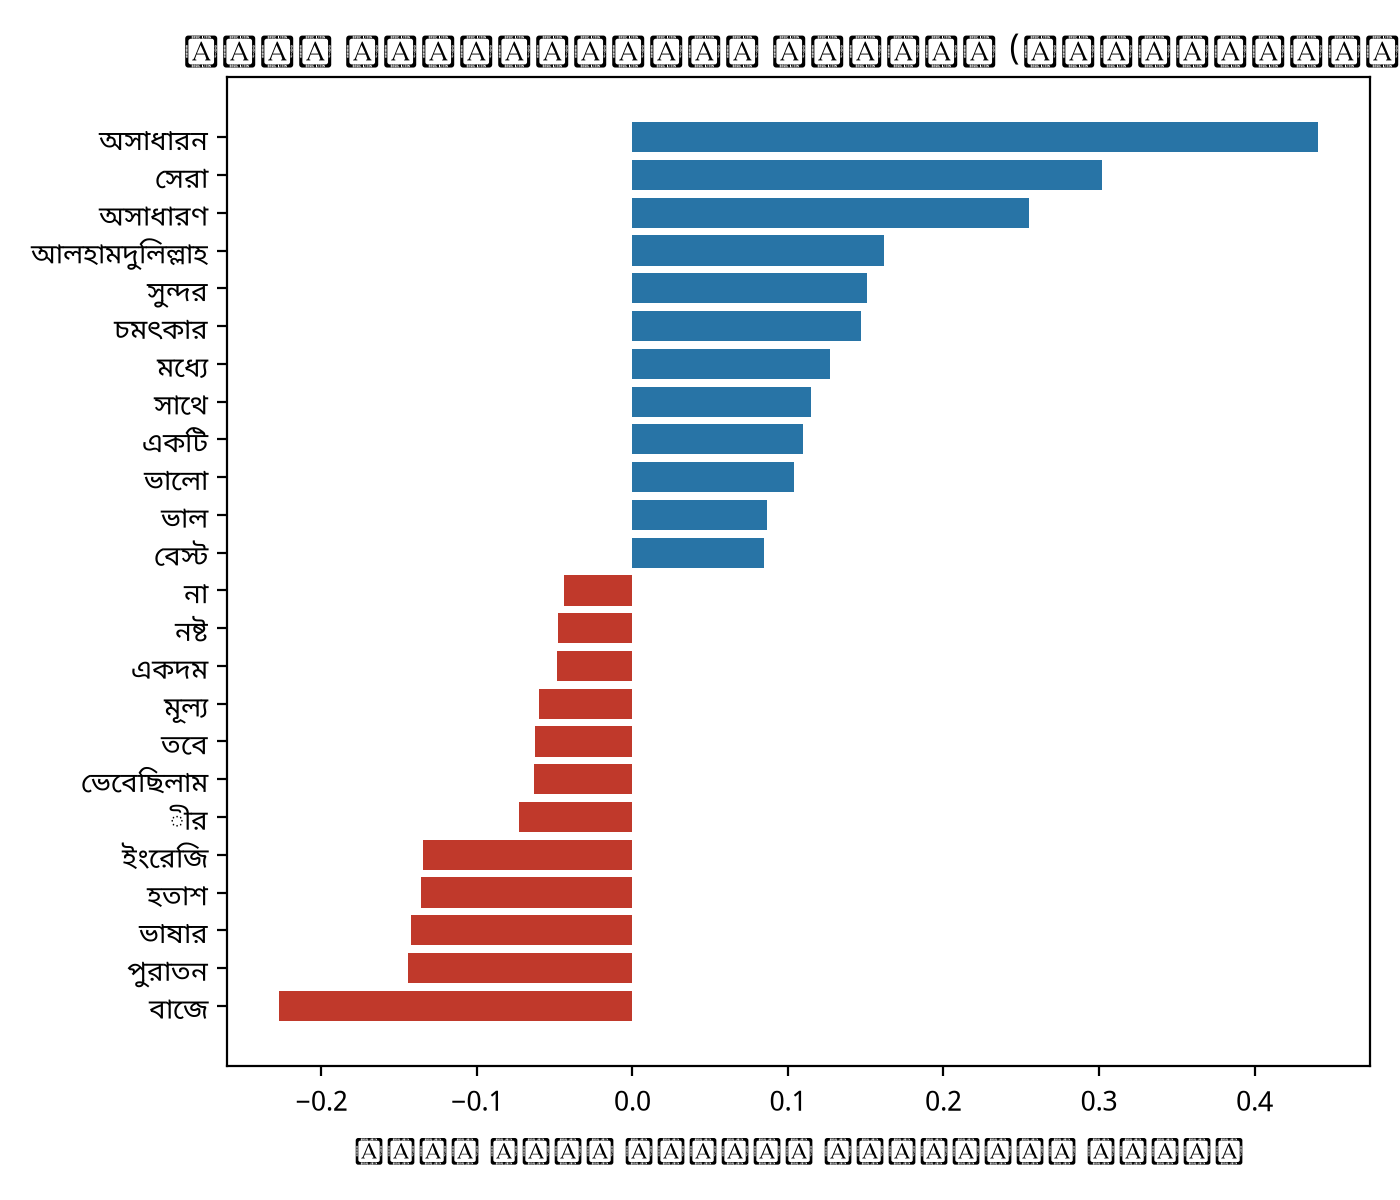
\includegraphics[width=\columnwidth]{fig5_shap.png}
\caption{Tokens with the largest mean SHAP contribution toward the positive class (60 held-out reviews; red: negative, blue: positive).}
\label{fig:shap}
\end{figure}
\begin{figure}[t]
\centering
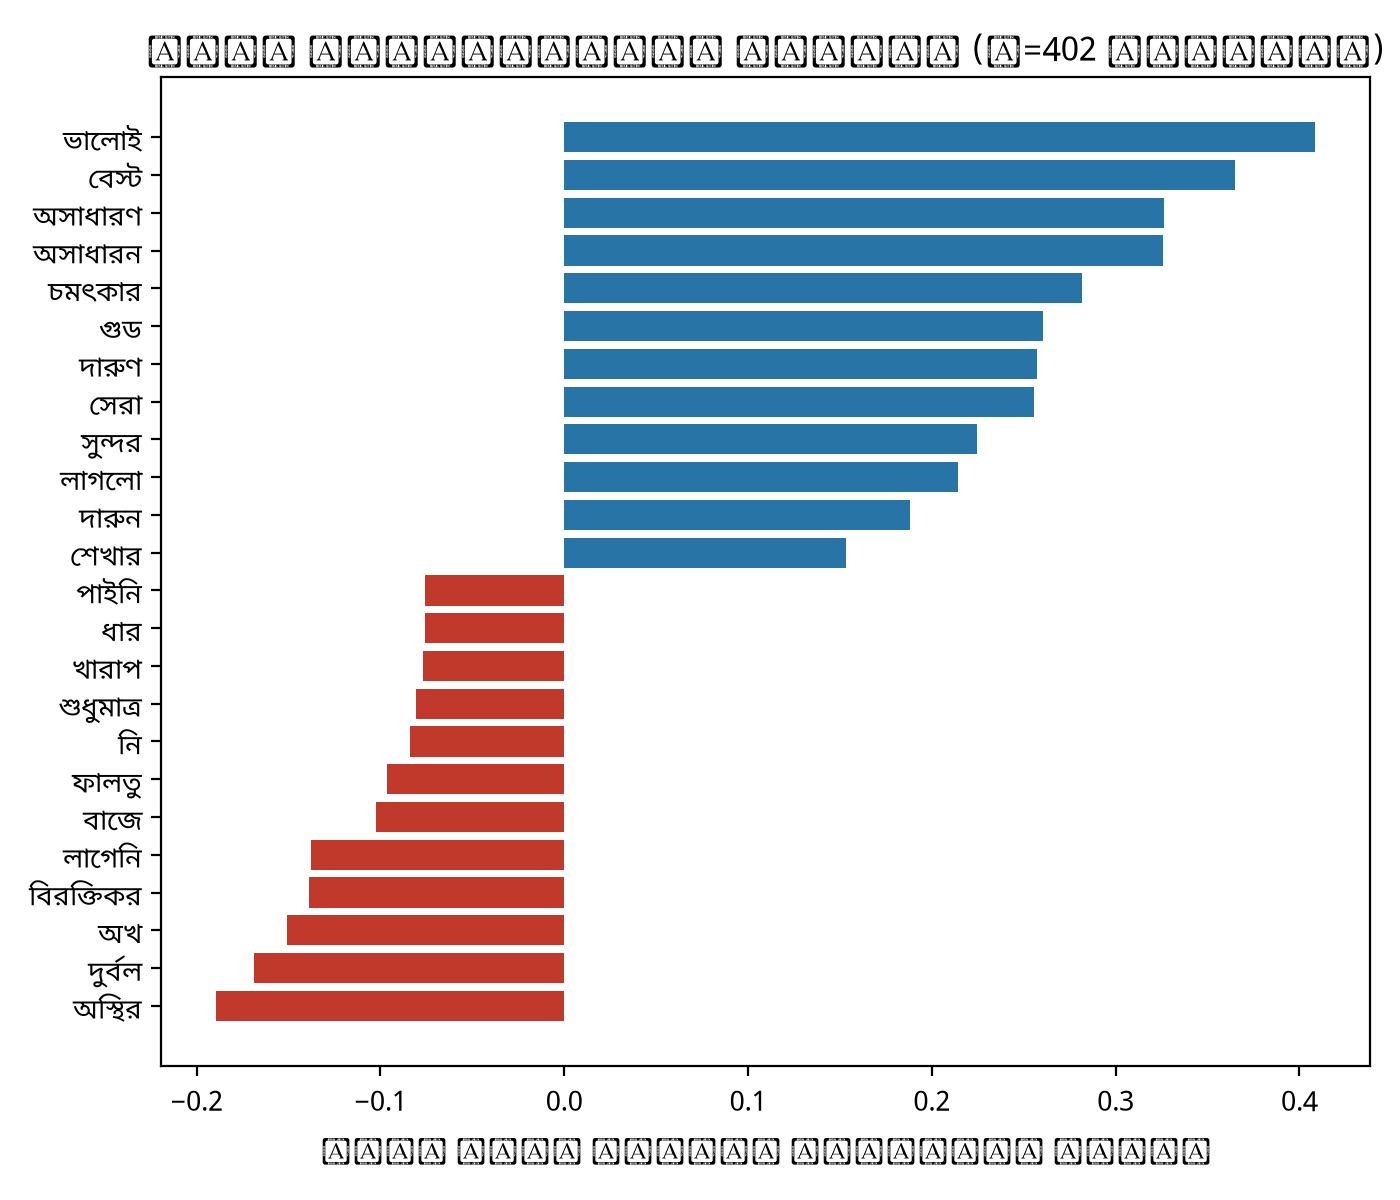
\includegraphics[width=\columnwidth]{fig6_shap_all402.png}
\caption{As Fig.~\ref{fig:shap}, computed on all 402 held-out reviews.}
\label{fig:shap402}
\end{figure}

\subsection{Cross-Source Transfer and External Validation}
An external collection of 6{,}541 reviews crawled from Rokomari \cite{sarker2022} was cleaned (5{,}277 reviews) and every cross-validated model was applied to it without further training. BanglaBERT reached $73.0\pm1.2$\% and BanglaBERT-large $73.5\pm0.8$\%, while the recurrent models reached 55--61\%. Part of the gap is label noise: ratings are only a proxy for sentiment, and Table~\ref{tab:ext} shows a review such as \bn{আলহামদুলিল্লাহ ভালো} (praise) with rating 0 labelled negative.

We also trained BanglaBERT on one source and tested it on the others (single seed; texts shared between sources removed from training). Mendeley $\rightarrow$ Rokomari gave 84.5\% accuracy (macro-F1 84.3\%), Rokomari $\rightarrow$ Mendeley 91.2\% (90.3\%); transfer to the 595 BanglaBook-derived reviews was poor (77.0\% and 82.4\%; macro-F1 58.3\% and 63.8\%), consistent with their rating-derived labels and the source--label confound.

\begin{table}[t]
\centering
\caption{Sample entries from the external dataset.}
\label{tab:ext}
\small
\begin{tabular}{lcc}
\toprule
Review & Rating & Label \\
\midrule
\bn{যারা ছোট বেলায় ক্রিকেট খেলছেন...} & 5 & Positive \\
\bn{আলহামদুলিল্লাহ ভালো} & 0 & Negative \\
\bn{গুড জব} & 1 & Negative \\
\bottomrule
\end{tabular}
\end{table}

\subsection{Official BanglaBook Benchmark}
On the official three-class BanglaBook split (110{,}645 training, 15{,}806 validation and 31{,}614 test reviews) a single BanglaBERT-large run with square-root class weights reached 91.87\% weighted F1. An unweighted two-epoch run reached 89.20\%, and a four-epoch run with maximum length 192 collapsed to the majority class (84.65\%); these earlier runs were adjusted after seeing test scores and are reported only for completeness. We then fixed the protocol and selected everything on the validation set: three runs (BanglaBERT-large with learning rate $10^{-5}$ without class weights, BanglaBERT-large with $1.5\times10^{-5}$ and square-root class weights, and BanglaBERT base) reached validation weighted F1 of 0.926, 0.925 and 0.924 (test 0.925, 0.926 and 0.923). Their probability average, with class offsets tuned on the validation set, reached 0.927 weighted F1 on the test set (accuracy 93.46\%, macro-F1 0.685), evaluated once. This is 0.6 points below the 0.933 reported in \cite{kabir2023}, so we do not claim to match the published result. The neutral class remains weak (F1 0.37).

\section{Discussion}
Recurrent models trained from scratch on about 1{,}600 reviews are limited to 73--81\% accuracy and are unstable across folds, whereas a pretrained Bengali language model reaches 93.8--94.2\% with much lower variance. Strong TF-IDF baselines (up to 90.2\% on BBR-2009 and 94.2\% on Mendeley) outperform every recurrent model, so pretraining rather than recurrence or attention is the decisive factor. Bidirectional processing and attention gave small, inconsistent gains. Language-specific pretraining outperformed multilingual pretraining, and the larger BanglaBERT model brought no benefit on this small dataset. Single folds of the same model differ by 13 points, illustrating how fragile a single 400-review test set is. The lower external accuracy and the label-noise analysis show that within-dataset scores do not guarantee transfer across sources, and that rating-derived labels limit what any model can achieve on the BanglaBook-originated part.

\section{Limitations}
First, BBR-2009 is small and was assembled from two sources of different origin: 595 reviews come from rating-labelled BanglaBook (almost all negative), so source and label are partly confounded. Second, labels derived from star ratings are noisy, which also affects the external evaluation. Third, the Rokomari cross-validation used a single seed, and the differences between base, large and ensemble models are within one standard deviation. Fourth, comparison with published results is indicative only because splits and preprocessing differ, and on the official BanglaBook benchmark our result remains below the published one. Fifth, the label-noise audit used a single LLM annotator rather than independent human annotators, so the suspected errors are not confirmed ground-truth corrections. Sixth, XLM-R and multilingual BERT were tuned only over a small grid, and large language models (few-shot) were not tested.

\section{Conclusion}
This study benchmarked twelve recurrent configurations, nineteen classical TF-IDF classifiers and four pretrained transformers for Bengali book review sentiment classification under repeated stratified cross-validation. Recurrent models trained from scratch reached at most 81.08\% accuracy, and single folds of one model span 13 points, so a single split is unreliable. BanglaBERT reached \pmstd{93.84}{1.10}\% on BBR-2009 (93.81\% for BanglaBERT-large and 94.23\% for the ensemble, a non-significant gain), \pmstd{96.72}{1.19}\% on the Mendeley corpus and \pmstd{90.60}{0.72}\% on the Rokomari corpus. Explanations were shown to be faithful, and confident errors concentrate in rating-derived labels. We do not claim state-of-the-art performance: on the official BanglaBook benchmark our result is below the published one.

\section{Future Work}
Future work includes larger and more diverse Bengali book review datasets with manually verified labels, manual re-annotation of the suspected label errors by independent annotators, evaluation of other pretrained models and instruction-tuned large language models (including few-shot prompting), emoji-aware preprocessing, domain-adaptive pretraining, and calibrated confidence estimates.

\section*{Data and Code Availability}
The BBR-2009 text, labels, source flags, fold assignments and a datasheet will be released for non-commercial use under the licence of the more restrictive source (CC BY-NC-SA 4.0); code and experiment logs will be released with the paper. % add repository URL here

\section*{Acknowledgment}
The authors thank the creators of the Mendeley Bengali Book Reviews, BanglaBook and Rokomari review datasets for making their data available.

\bibliographystyle{IEEEtran}
\bibliography{refs}

\end{document}
